\documentclass[tikz, crop, border={0.2cm}]{standalone}%
\usepackage{drawstack}%
%
\begin{document}
  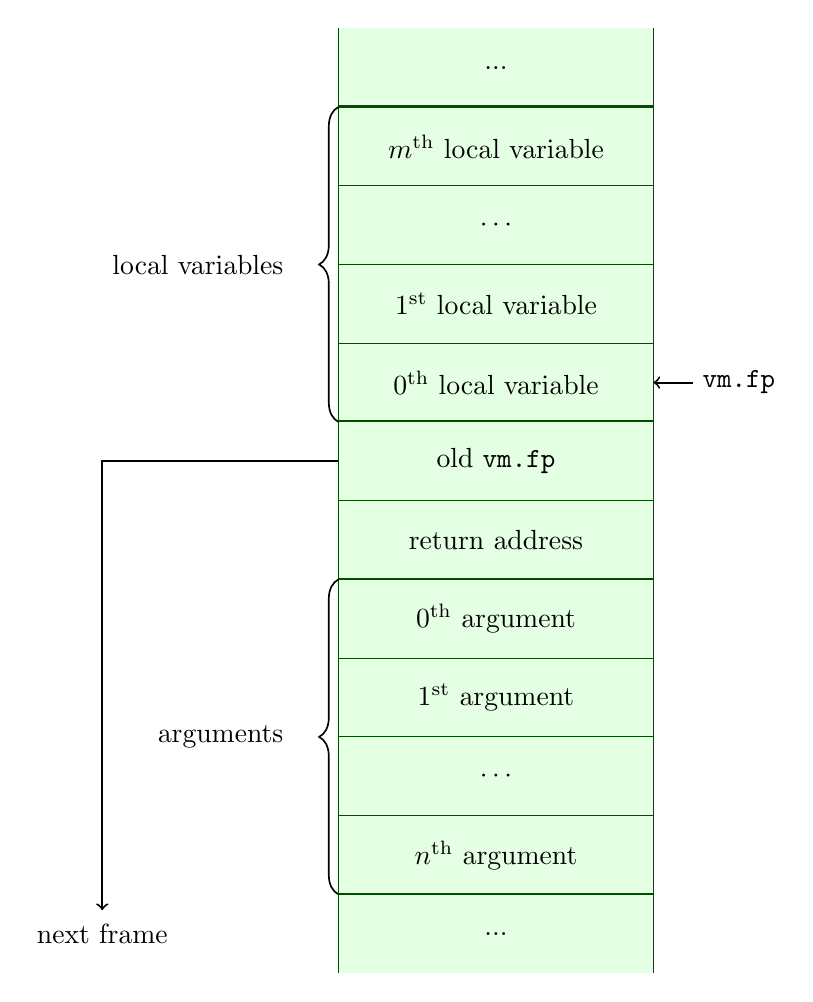
\begin{tikzpicture}
    \newcounter{fptr.mid}
    \setcounter{fptr.mid}{-5}
    \stacktop{}
    \separator
    \startframe
    \cell{$m^\mathrm{th}$ local variable}
    \cell{$\cdots$}
    \cell{$1^\mathrm{st}$ local variable}
    \cell{$0^\mathrm{th}$ local variable}
      \cellptr{{\ttfamily vm.fp}}
    \finishframe{local variables}
    \separator
    \cell{old {\ttfamily vm.fp}}
      \coordinate (old_fp_A) at (-2, \value{cellnb});
      \coordinate (old_fp_B) at (\value{fptr.mid}, \value{cellnb});
    \cell{return address}
    \separator
    \startframe
    \cell{$0^\mathrm{th}$ argument}
    \cell{$1^\mathrm{st}$ argument}
    \cell{$\cdots$}
    \cell{$n^\mathrm{th}$ argument}
    \finishframe{arguments}
    \separator
    \stackbottom{}
    \draw (\value{fptr.mid}, \value{cellnb}) node {next frame};
      \coordinate (old_fp_C) at (\value{fptr.mid}, \value{cellnb} + 0.3);
    \draw[->, line width=0.7pt] (old_fp_A) -- (old_fp_B) -- (old_fp_C);
  \end{tikzpicture}
\end{document}
